\section{Side by side comparison between both analysis results}
\label{sec:sidebyside}
\vspace{-85px}
\begin{figure}[H]
\hspace{-10mm}
  \subfigure[Theoretical analysis]{% 
    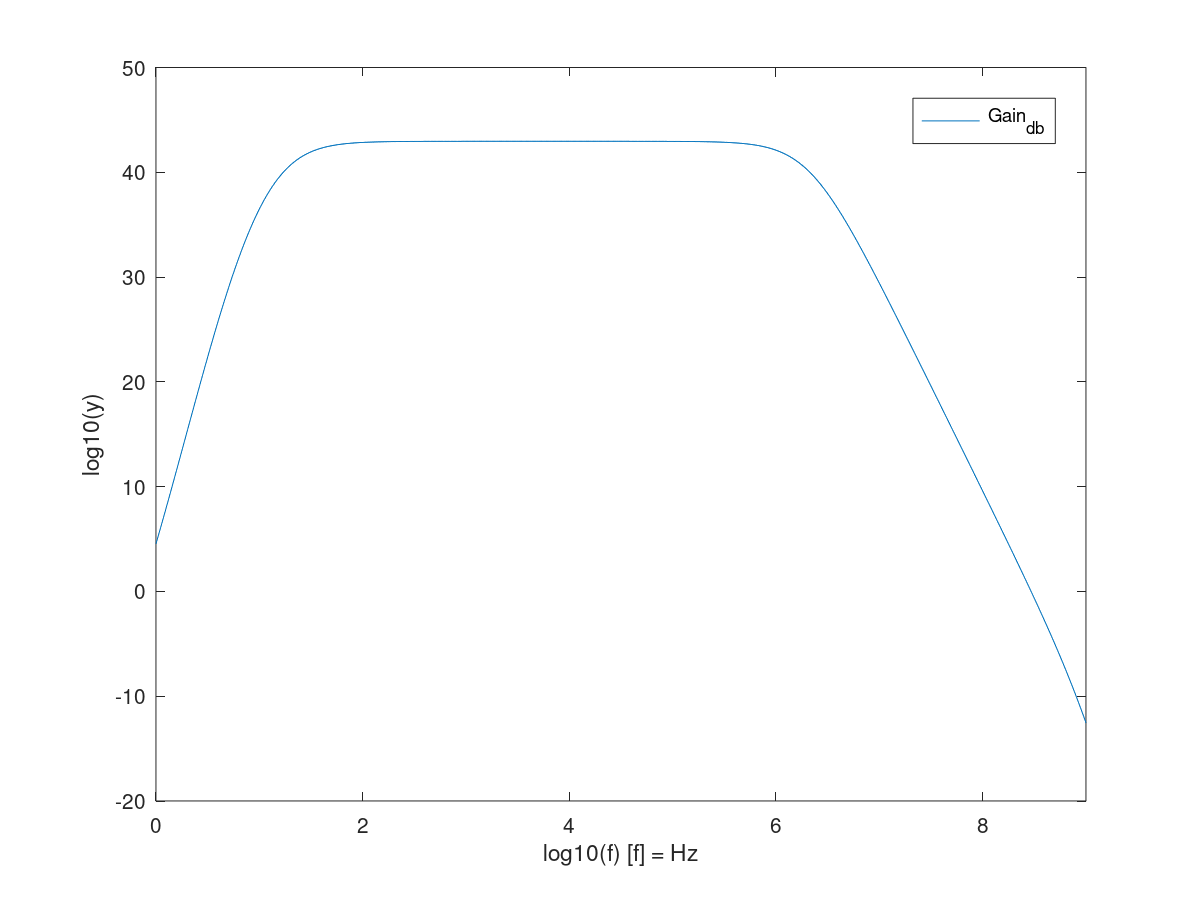
\includegraphics[width=.66\textwidth]{../mat/gaindb.png}
  } 
  \hspace{-30px}
  \subfigure[Simulation analysis]{% 
    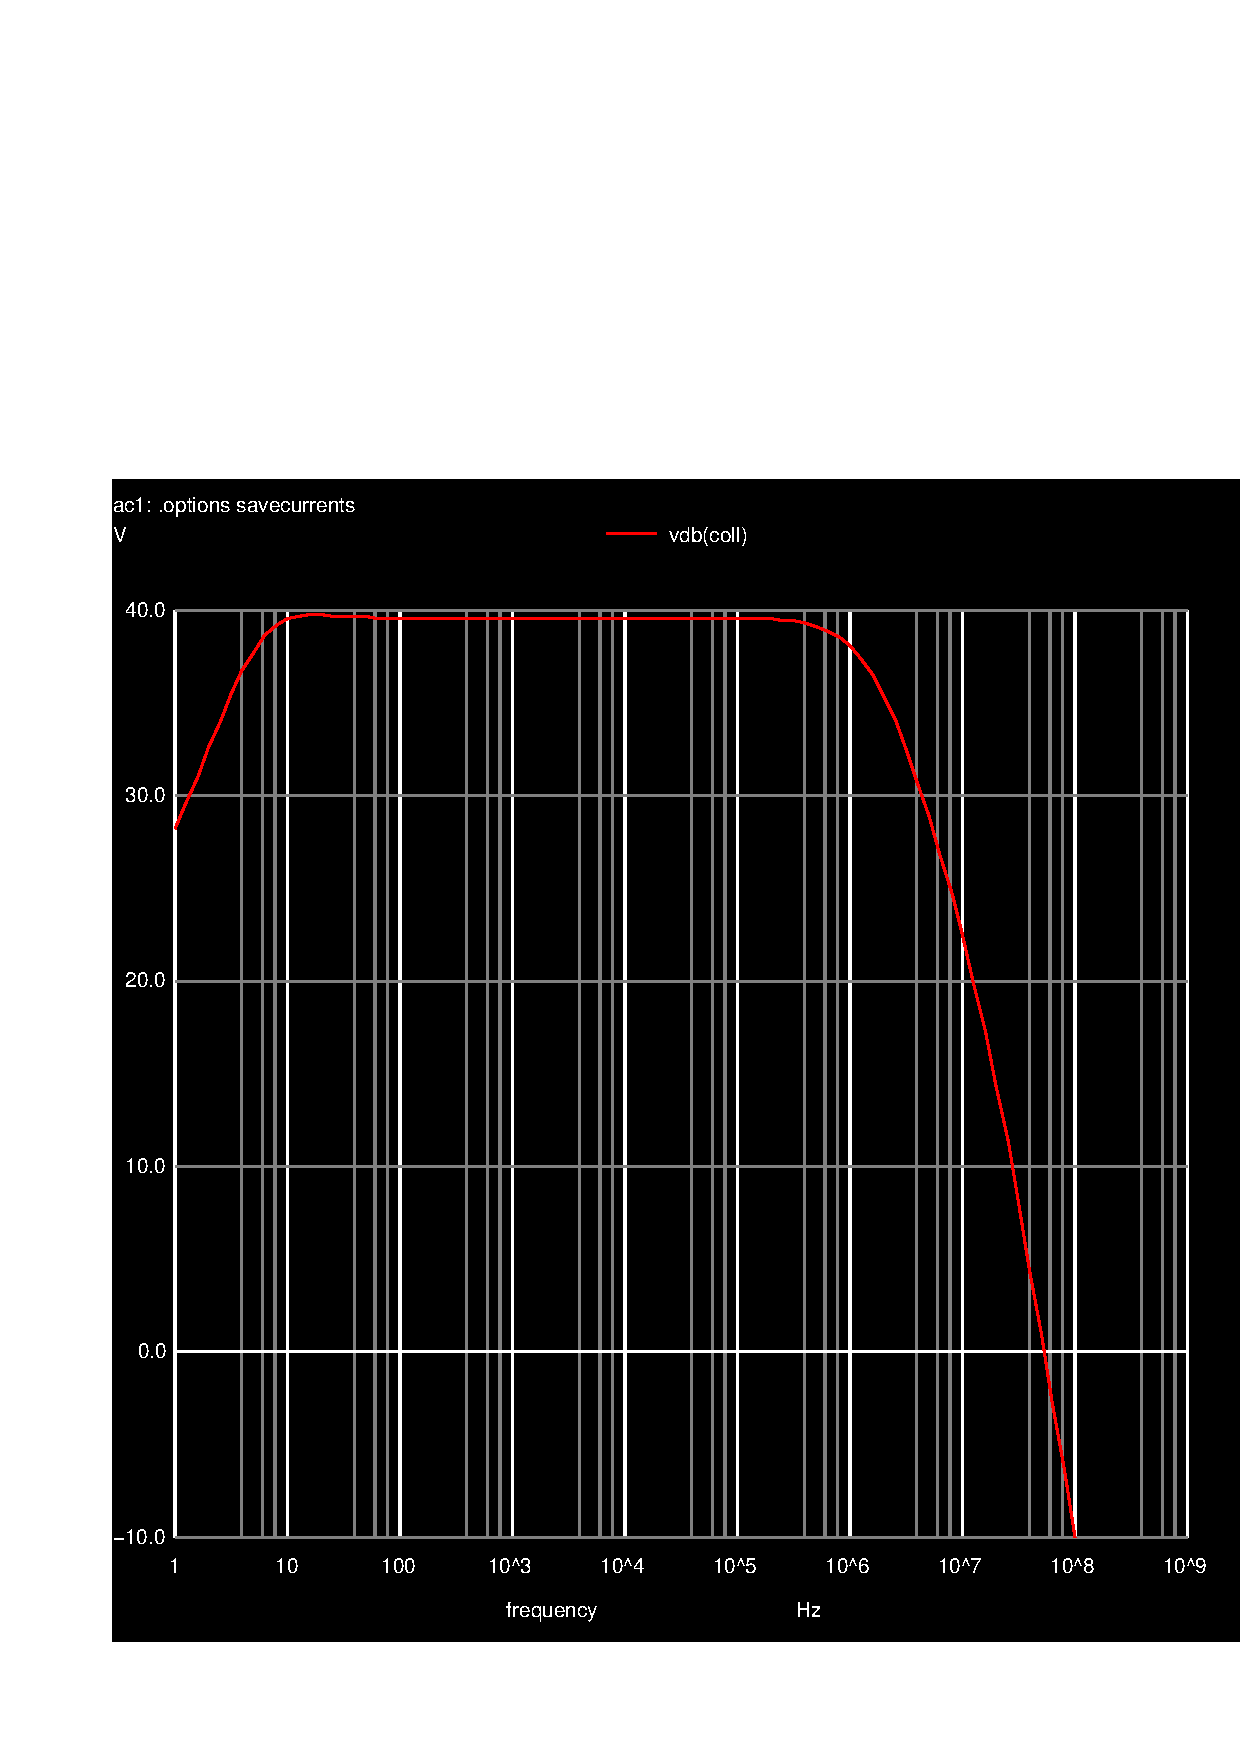
\includegraphics[width=.45\textwidth]{../sim/gainplotdb.pdf}
  } 
  \caption{Comparison between the obtained plots for the gain stage output dB voltage on \textit{Ngspice} and \textit{Octave}} 
\end{figure}

Once the linear approximation for the transistors were the version with the capacitors the shape of the curves are similar but there are still differences, specifically the theoretical analysis predicts an gain voltage in dB of above 40 as the simulation predicts slightly bellow 40. The other considerable difference is for the higher frequency that both expect very low gains but the simulation analysis decreases faster.

\vspace{-75px}
\begin{figure}[H]
\hspace{-10mm}
  \subfigure[Theoretical analysis]{% 
    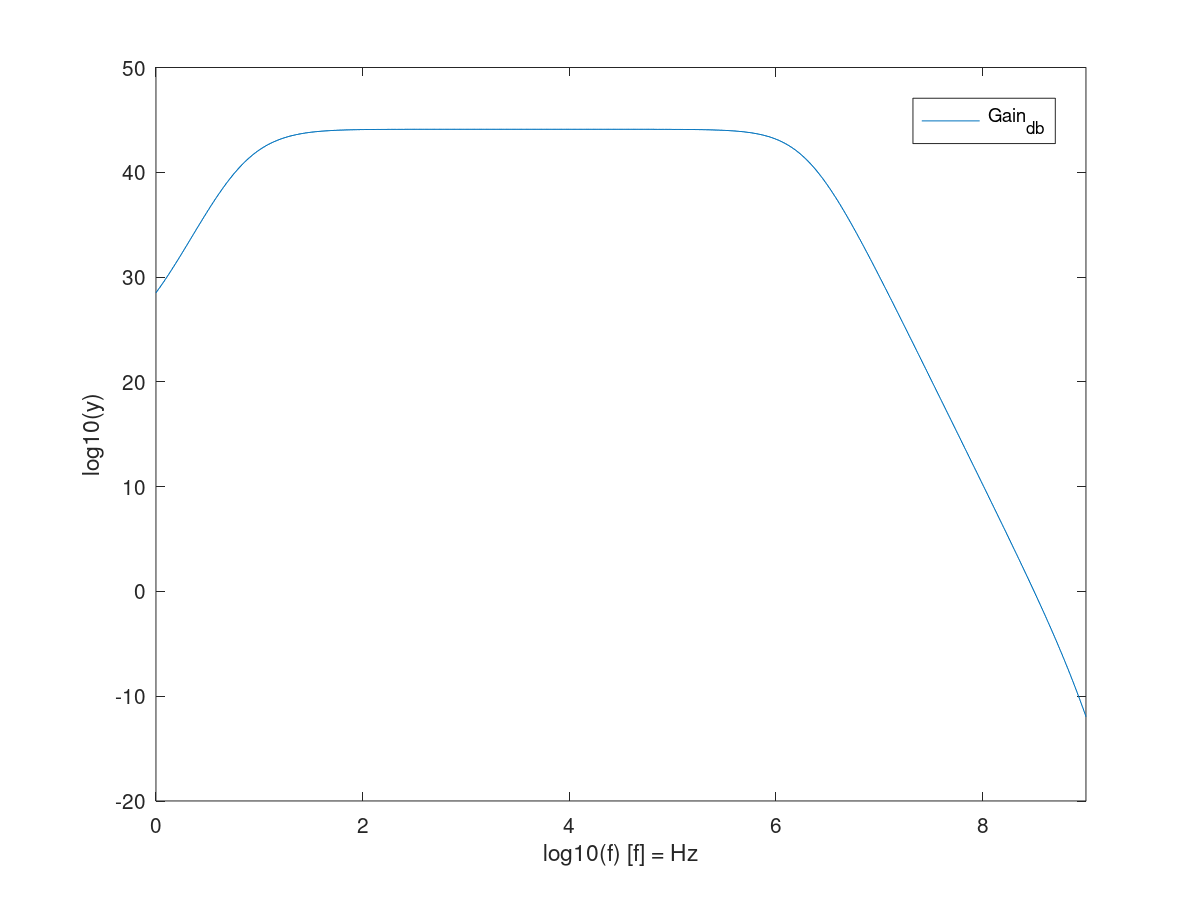
\includegraphics[width=.66\textwidth]{../mat/gaindb_coll.png}
  } 
    \hspace{-30px}
  \subfigure[Simulation analysis]
  {% 
    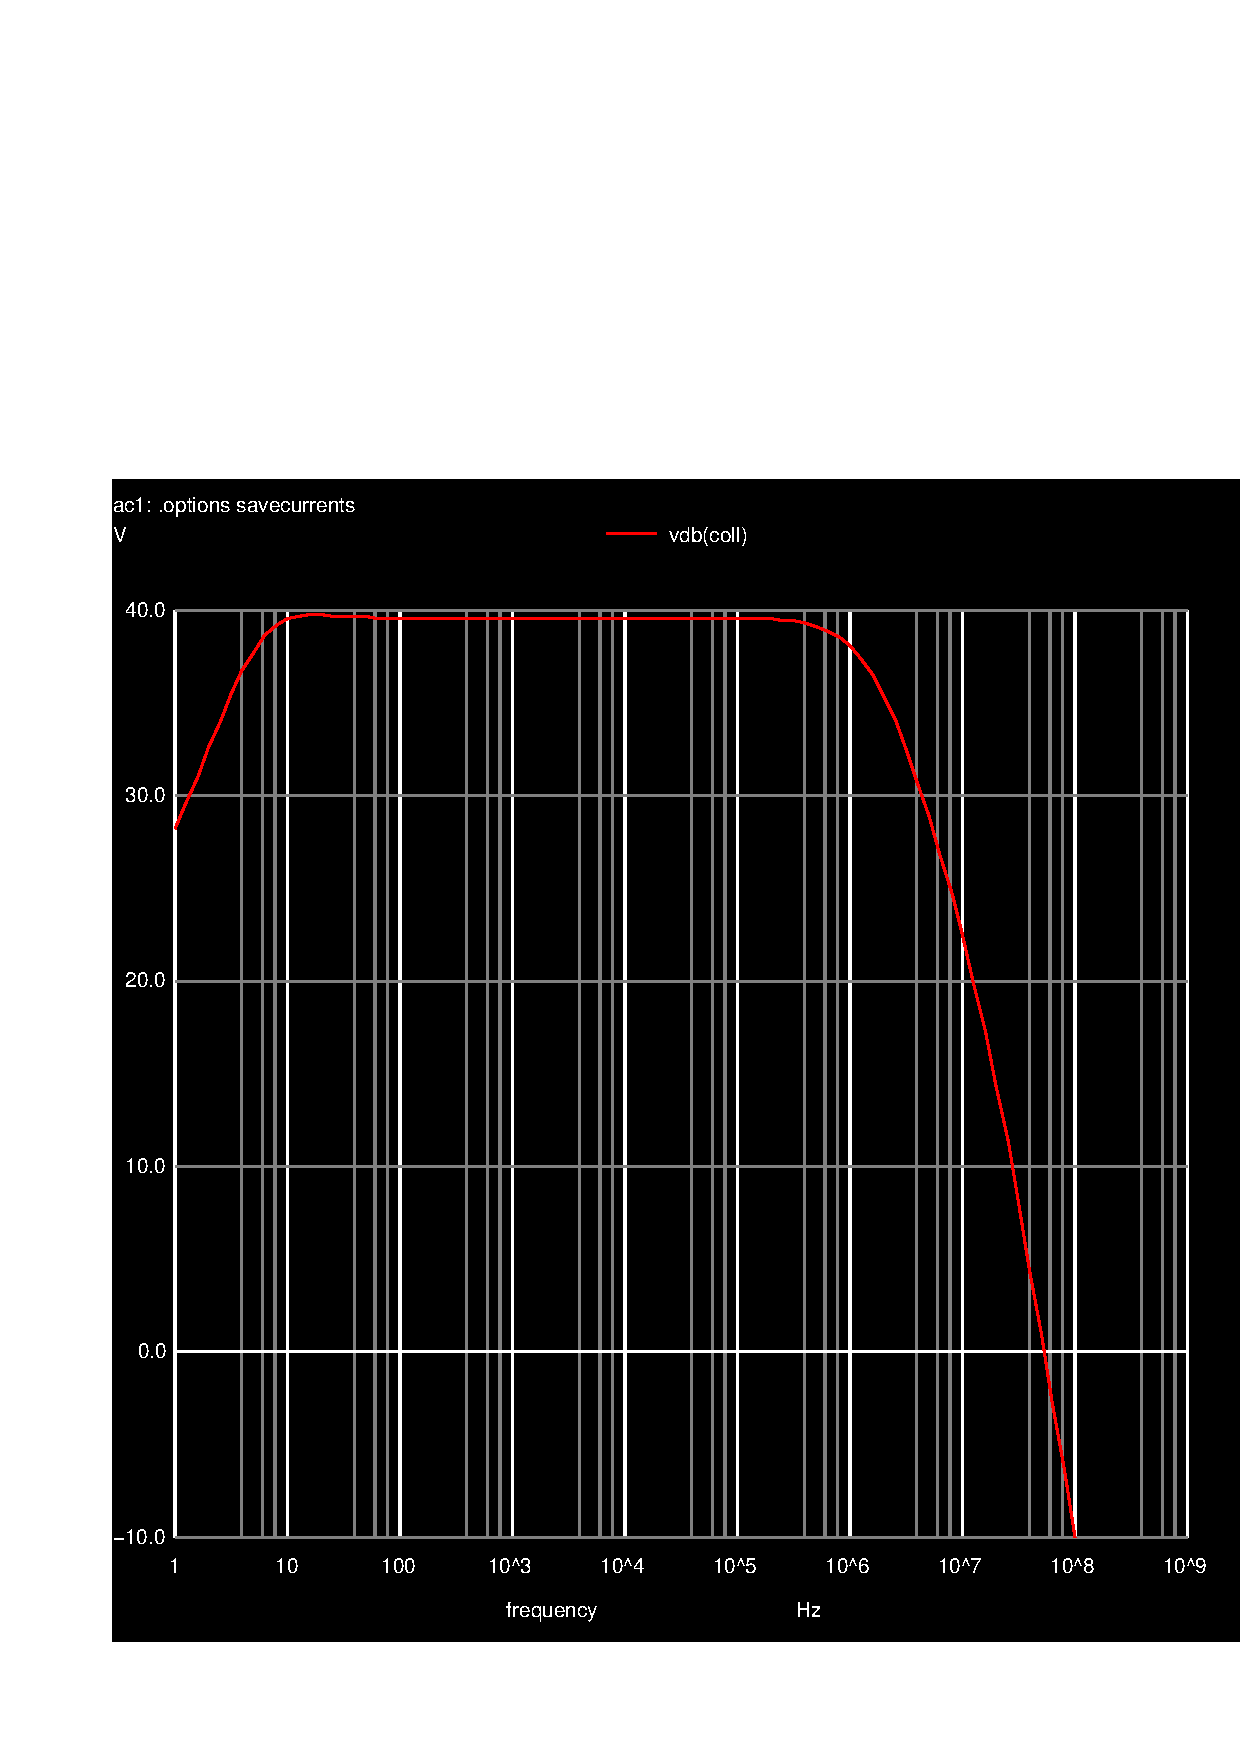
\includegraphics[width=.45\textwidth]{../sim/gainplotdb.pdf}
  } 
  \caption{Comparison between the obtained plots for the circuit output dB voltage on \textit{Ngspice} and \textit{Octave}} 
\end{figure}

Between the gain stage and the output stage the signal maintains the shift for above 40 in the theoretical analysis, but the difference for the higher frequencies seems to be attenuated. This is to be expected but 



\begin{table}[H]
    \begin{minipage}{.5\textwidth}
    \centering
    \vspace{3mm}
    \begin{table}[H]
    \centering
        \centering
        \begin{tabular}{c|c}
        \textbf{Quantity} & \textbf{Value}\\
    Gain & $146.663979$\\ \hline 
Gain (dB) & $43.326469$\\ \hline 
Lower cut-off frequency & $14.307230$ Hz\\ \hline 
Higher cut-off frequency & $1668100.537200$ Hz\\ \hline 
Bandwidth & $1668086.229970$ Hz\\ \hline 
Cost & $3278.058000$ MU\\ \hline 
Merit & $5216.386618$\\ \hline 
|Zi| & $6171.629952 \Omega$ \\ \hline 
|Zo| & $9.152525 \Omega$ \\ \hline 

    \hline
    \end{tabular}
    \label{tab:quantities_side_octave}
    \end{table}
    \vspace{6mm}
    \caption{Theoretical analysis.}
    \end{minipage}
    \begin{minipage}{.5\textwidth}
        \begin{table}[H]
        \centering
        \begin{tabular}{c|c}
        \textbf{Quantity} & \textbf{Value}\\
        \hline
        \hline
        Gain & 73.2378 V\\ \hline
Gain (dB) & 37.2947 dB\\ \hline
Lower cut-off frequency & 12.5855 Hz\\ \hline
Upper cut-off frequency & 1.57176E+06 Hz\\ \hline
Bandwidth & 1.57175E+06 Hz\\ \hline
Cost & 3278.06 MU\\ \hline
Merit & 2790.17\\ \hline

        Zi & 1385.89 + (-36.7344)j $\Omega$\\ \hline
|Zi| & 1386.38 $\Omega$\\ \hline

        Zo & 14.0507 + (0.625162)j $\Omega$\\ \hline
|Zo| & 14.0646 $\Omega$\\ \hline

    \end{tabular}
        \caption{Simulation analysis}
        \label{tab:quantaties_side_ngspice}
    \end{table}
    \end{minipage}
    \caption{Relevant values for our goals.} 
\end{table}

The differences in the gain and in the input impedance cannot be ignored. These may come from the approximations done in the  theoretical analysis when we totally ignore the capacitors contribution. Furthermore, we also use a 8x8 matrix, which might easily introduce numerical errors. Thus, because the rest of the values are around the same magnitude, we feel that it is a good result overall, given the nonlinear aspect of the transistor. One last comment, because our OP, although sufficient for us to be working in the FAR, is close to $V_{beon}$ (it is so in order to increase our merit), which might make the transistor, in the Ngspice model, to start to behave differently than from our analysis through Octave. 